\documentclass[class=article, crop=false, 12pt]{standalone}
\usepackage[subpreambles=true]{standalone}
\usepackage{../.common/common}


\author{Tony Shing}
%\pretitle{Supplementary}

\topic{Note 2B (Math for Physics)}
\title{Non-Cartesian Coordinate}

\version{2025} % leave blank for omitting

\begin{document}

\maketitle

%\heading{Lecture}{Tony}

\begin{overview}
    \begin{itemize}
        \item 2D: Polar coordinate
        \item 3D: Cylindrical coordinate \& Spherical coordinate
    \end{itemize}
\end{overview}



% content begins here
% Section %%%%%%%%%%%%%%%%%%%%%%%%%%%%%%%%%%%%%%%%%%%%%%%%%%%%
\section{Polar Coordinate}

You should have already learnt what polar coordinate is from high school,
and its conversion with rectangular coordinate.

\begin{center}
    \begin{minipage}{0.4\textwidth}
        \centering
        \ul{From $(x,y)$ to $(r,\theta)$}
        \\[1em]
        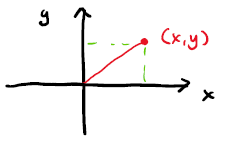
\includegraphics[height=7em]{xy}
        \\[-2em]
        \aleq{
            \bcase{
                r &= \sqrt{x^2+y^2}\\
                \theta &= \tan^{-1}{\qty(\dfrac{y}{x})}
            }
        }
    \end{minipage}
    %
    \begin{minipage}{0.4\textwidth}
        \centering
        \ul{From $(r,\theta)$ to $(x,y)$}
        \\[1em]
        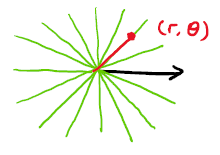
\includegraphics[height=7em]{polar}
        \\[-2em]
        \aleq{
            \bcase{
                x &= r\cos\theta\\
                y &= r\sin \theta
            }
        }
    \end{minipage}
\end{center}


What about double integral over an area that is represented by polar coordinate?

\aleq{
    \Aboxed{
        \iint f(x,y)\dd{x}\dd{y} \quad\Leftrightarrow\quad \iint f(r,\theta)\, \tkn{extraR}{\cul[red]{r}}\dd{r}\dd{\theta}
    }
}\\
\addArrow[red]{extraR}{(0,-4ex)}{Caution: An extra $r$}{(0,-1ex)}





The reason for this extra $r$ comes from the dimension of the area element.

\begin{itemize}
    \item In $x/y$ coordinate, area of each grid is fixed.
    
    \begin{minipage}{0.7\textwidth}
        \aleq{
            I = \sum_i \tkn{weightxy}{\cul[red]{f(x_i, y_i)}} \cdot \tkn{Axy}{\cul[blue]{\Delta x\Delta y}} \sim \iint f(x,y)\dd{x}\dd{y}
        }\\
        \addArrow[red]{weightxy}{(-4ex,-3ex)}{"Weight" assigned \\ to the point $(x_i,y_i)$}
        {(0,-2ex)}{(-2ex,-2ex)}
        \addArrow[blue]{Axy}{(4ex,-3ex)}{Each grid are\\ of area $\Delta x\Delta y$}
        {(0,-2ex)}{(2ex,-2ex)}
    \end{minipage}
    %
    \begin{minipage}{0.28\textwidth}
        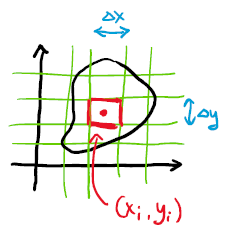
\includegraphics[width=0.75\textwidth]{xy_grid}
    \end{minipage}
    

    \item In polar coordinate, area of the grids depends on its $r$ coordinate.
    When $\Delta \theta$ is very small, 
    the grid's area $\approx$ (height)$\times$(width) $\approx \Delta r\times r_i\Delta \theta$. So

    \begin{minipage}{0.6\textwidth}
        \aleq{
            I = \sum_i \tkn{weightpo}{\cul[red]{f(r_i, \theta_i)}} \cdot \tkn{Apo}{\cul[blue]{r_i \cdot \Delta r\Delta \theta}} \sim \iint f(r,\theta)r\dd{r}\dd{\theta}
        }\\
        \addArrow[red]{weightpo}{(-4ex,-3ex)}{"Weight" assigned \\ to the point $(r_i,\theta_i)$}
        {(0,-2ex)}{(-2ex,-2ex)}
        \addArrow[blue]{Apo}{(6ex,-3ex)}{The grid's area \\ depends on $r$ coordinate \\ $= \Delta r \times r_i \Delta \theta$}
        {(0,-2ex)}{(2ex,-3.5ex)}
    \end{minipage}
    %
    \begin{minipage}{0.38\textwidth}
        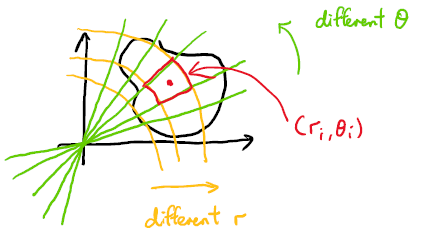
\includegraphics[width=\textwidth]{polar_grid}
    \end{minipage}

    \hfill\\[1em]
    \begin{center}
        \begin{minipage}{0.3\textwidth}
            \centering
            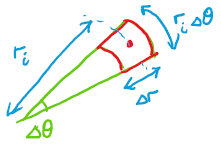
\includegraphics[width=0.8\textwidth]{polar_arc}
        \end{minipage}
        %
        \begin{minipage}{0.4\textwidth}
            \centering
            \red{\ul{
                Each grid's area depends}\\
                \ul{on its $r$ coordinate.
            }}\\[1em]
            When $\Delta \theta$ is very small,\\
            grid's area $\approx$ (height)$\times$(width)\\
            \hspace{7.5ex}$\approx (\Delta r) \times (r\Delta \theta)$
        \end{minipage}
    \end{center}

\end{itemize}


\linesep
% Section %%%%%%%%%%%%%%%%%%%%%%%%%%%%%%%%%%%%%%%%%%%%%%%%%%%%
\section{Cylindrical Coordinate}

Cylindrical coordinate is essentially polar coordinate + z-axis.

\begin{center}
    \begin{minipage}{0.4\textwidth}
        \centering
        \ul{From $(x,y,z)$ to $(r,\theta,z)$}
        \\[1em]
        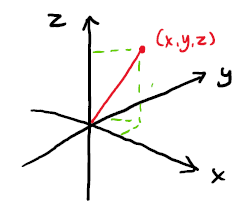
\includegraphics[height=7em]{xyz}
        \\[-2em]
        \aleq{
            \bcase{
                r &= \sqrt{x^2+y^2}\\
                \theta &= \tan^{-1}{\qty(\dfrac{y}{x})}\\
                z &= z
            }
        }
    \end{minipage}
    %
    \begin{minipage}{0.4\textwidth}
        \centering
        \ul{From $(r,\theta,z)$ to $(x,y,z)$}
        \\[1em]
        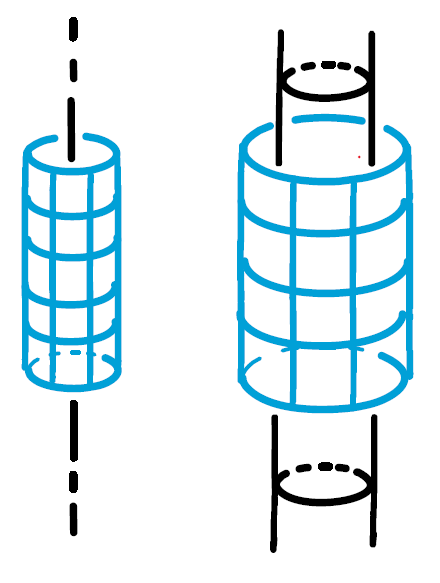
\includegraphics[height=7em]{cyl}
        \\[-2em]
        \aleq{
            \bcase{
                x &= r\cos\theta\\
                y &= r\sin \theta \\
                z &= z
            }
        }
    \end{minipage}
\end{center}




Therefore the triple integral expression is very similar to the double integral in polar coordinate,
with an extra $r$ present in the volume element.
\aleq{
    \Aboxed{
        \iiint f(x,y,z)\dd{x}\dd{y}\dd{z} \quad\Leftrightarrow\quad \iiint f(r,\theta,z)\, \cul[red]{r}\dd{r}\dd{\theta}\dd{z}
    }
}

\begin{center}
    \begin{minipage}{0.3\textwidth}
        \centering
        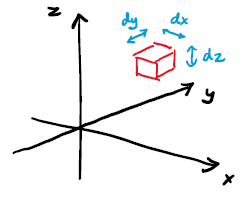
\includegraphics[height=7em]{xyz_unit}
    \end{minipage}
    %
    $\Leftrightarrow$
    %
    \begin{minipage}{0.3\textwidth}
        \centering
        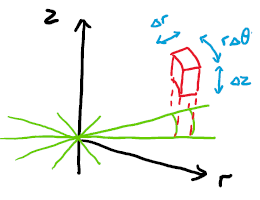
\includegraphics[height=7em]{cyl_unit}
    \end{minipage}
\end{center}


\begin{example}
    Given a solid cylinder with mass density distribution $\rho(r,\theta,z) = r^2$,
    and dimension: radius = $R$, height = $H$. 
    Making use of cylindrical coordinate,
    \begin{itemize}
        \item Mass of each volume element = (density)$\times$(volume) $= \rho(r,\theta,z)r\dd{r}\dd{\theta}\dd{z}$
        \item Total mass $= \iiint \rho(r,\theta,z) r\dd{r}\dd{\theta}\dd{z}$
    \end{itemize}

    \begin{minipage}{0.7\textwidth}
         \begin{itemize}
            \item Upper/Lower bound for each dimension are:
            \begin{itemize}
                \item Range of $r$: From $r=0$ to $r=R$
                \item Range of $\theta$: From $\theta=0$ to $\theta = 2\pi$ (whole circle)
                \item Range of $z$: From $z=0$ to $z=H$
            \end{itemize}
        \end{itemize}
    \end{minipage}
    \begin{minipage}{0.2\textwidth}
        \centering
        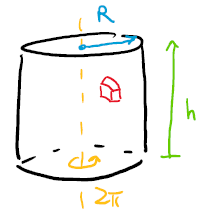
\includegraphics[height=7em]{cyl_eg}
    \end{minipage}
   
    \hfill\\[1em]
    The calculaton of the total mass is then
    \aleq{
        &\int_{z=0}^{z=H}\int_{r=0}^{r=R}\int_{\theta=0}^{\theta=2\pi} \tkn{r2}{\red{\ul{r^2}}} \cdot r\dd{\theta}\dd{r}\dd{z}\\[1em]
        = &\int_{z=0}^{z=H}\int_{r=0}^{r=R} \cub[yellow]{\qty(\int_{\theta=0}^{\theta=2\pi} r^3\dd{\theta})}{\text{First integrate }\theta}\dd{r}\dd{z} \\[1em]
        = &\int_{z=0}^{z=H}\int_{r=0}^{r=R} \qty[r^3\theta]\eval_{\theta=0}^{\theta=2\pi} \dd{r}\dd{z} \\[1em]
        = &\int_{z=0}^{z=H} \cub[blue]{\qty(\int_{r=0}^{r=R} 2\pi r^3\dd{r})}{\text{Then integrate }r}\dd{z} \\[1em]
        = &\int_{z=0}^{z=H}\qty[\frac{2\pi r^4}{4}]\eval_{r=0}^{r=R} \dd{z} \\[1em]
        = &\cub[green]{\int_{z=0}^{z=H} \frac{\pi R^4}{2} \dd{z}}{\text{Finally integrate }z} \\[1em]
        = & \frac{\pi R^4 H}{2}
    }
    \addArrow[red]{r2}{(4ex, 2ex)}{density function $\rho(r,\theta,z)=r^2$}
    {(2ex, 2ex)}{(12ex,1ex)}
\end{example}


\linesep
\newpage
% Section %%%%%%%%%%%%%%%%%%%%%%%%%%%%%%%%%%%%%%%%%%%%%%%%%%%%
\section{Spherical Coordinate}

Spherical coordinate is a description of position on a sphere by 3 parameters:
\begin{itemize}
    \item $r$ = Radius, $\sim$ Altitute
    \item $\theta$ = Polar angle, $\sim$ Latitude
    \item $\phi$ = Azimuthal angle, $\sim$ Longitude
\end{itemize}

The conversion to rectangular coordinate is as follow:

\begin{center}
    \begin{minipage}[t]{0.4\textwidth}
        \centering
        \ul{From $(x,y,z)$ to $(r,\theta,\phi)$}
        \\[1em]
        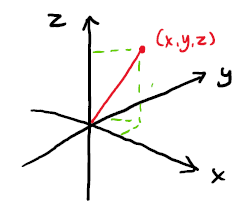
\includegraphics[height=7em]{xyz}
        \\[-2em]
        \aleq{
            \bcase{
                r &= \sqrt{x^2+y^2+z^2}\\
                \theta &= \tan^{-1}{\qty(\dfrac{\sqrt{x^2+y^2}}{z})} \\[1.1em]
                \phi &= \tan^{-1}{\qty(\dfrac{y}{x})}
            }
        }
    \end{minipage}
    %
    \begin{minipage}[t]{0.4\textwidth}
        \centering
        \ul{From $(r,\theta, \phi)$ to $(x,y,z)$}
        \\[1em]
        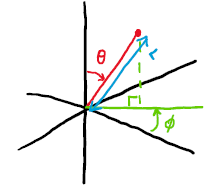
\includegraphics[height=7em]{sph}
        \\[-2em]
        \aleq{
            \bcase{
                x &= r\sin\theta\cos\phi\\
                y &= r\sin\theta\sin\phi \\
                z &= r\cos\theta
            }
        }
    \end{minipage}
\end{center}



\ul{Caution 1:} \red{The notations here are adopting the \bf{physics convention}}, 
where $\phi$ is the angle on the $x$-$y$ plane and $\theta$ is the inclination to the $z$-axis.
This is the convention found in modern Physics textbooks. 
However in many mathematics textbook and older physics books, 
you may find the \red{\bf{mathematics convention}
where the meaning of $\phi$ and $\theta$ are swapped.}\\

\ul{Caution 2:} The choice of the angles are not the same as we use geography. Note that\\

\begin{minipage}{0.7\textwidth}
    \begin{itemize}
        \item Range of $\theta = [0,\pi]$. But in geography, 
        latitude angle is $90\degree-\theta$, which ranged between $[-90\degree, 90\degree]$.

        \item Range of $\phi = [0, 2\pi)$. But in geography, 
        longitutude is ranged between $(-180\degree, 180\degree]$.
        
    \end{itemize}
\end{minipage}
%
\begin{minipage}{0.28\textwidth}
    \centering
    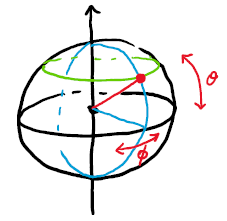
\includegraphics[height=6em]{gps}
\end{minipage}

\hfill\\[1em]
When dealing with triple integral, 
the unit volume in spherical coordinate is $\sim (\Delta r)\times(r\Delta \theta)\times(r\sin\theta\Delta \phi)$.
We may visualize as follows:

\addBentArrow*{unitcell}{(24ex,-3ex)}{}{(28ex,6ex)}
\addBentArrow*{watermelon}{(-25ex,4ex)}{}{(-26ex,-6ex)}
\begin{center}
    \tkm{unitcell}
    \begin{minipage}{0.3\textwidth}
        \centering
        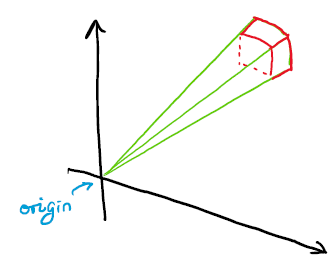
\includegraphics[height=9em]{sph_unit}
    \end{minipage}
    %
    \begin{minipage}{0.3\textwidth}
        \centering
        Volume element\\
        = Skin of a watermelon cone
    \end{minipage}
    %
    \begin{minipage}{0.3\textwidth}
        \centering
        
\includegraphics[height=9em]{watermelon.jpg}
    \end{minipage}
    \tkm{watermelon}
\end{center}

\begin{center}
    \begin{minipage}{0.4\textwidth}
        \centering
        \ul{The side along $r$ direction: $\dd{r}$}\\[0.5em]
        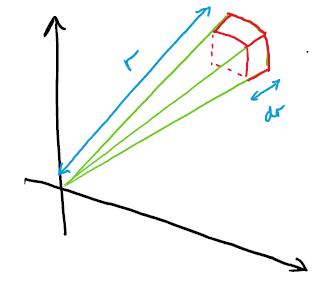
\includegraphics[height=11em]{sph_unit_r}
    \end{minipage}
    %
    \begin{minipage}{0.4\textwidth}
        \centering
        \ul{The side along $\theta$ direction: $r\dd{\theta}$}\\[0.5em]
        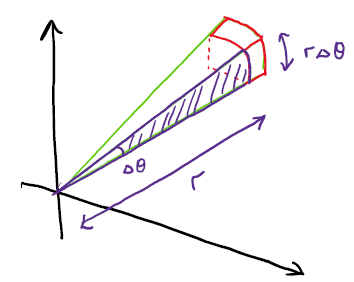
\includegraphics[height=11em]{sph_unit_th}
    \end{minipage}
\end{center}

\begin{center}
    \begin{minipage}{\textwidth}
        \ul{The side along $\phi$ direction: $r\sin{\theta}\dd{\phi}$}
    \end{minipage}
    %
    \hfill\\[1em]
    %
    \begin{minipage}{0.35\textwidth}
        \centering
        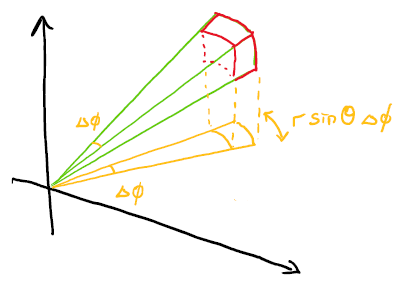
\includegraphics[height=11em]{sph_unit_ph}
    \end{minipage}
    %
    \begin{minipage}{0.35\textwidth}
        \centering
        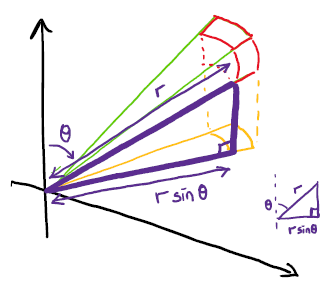
\includegraphics[height=11em]{sph_unit_ph2}
    \end{minipage}
    %
    \begin{minipage}{0.28\textwidth}
        \centering
        \purple{The radius is $r\sin\theta$, not $r$. \\ Because it is the radius's \\ projection}
    \end{minipage}
\end{center}


As a result, the triple integral has to be written as

\aleq{
    \Aboxed{
        \iiint f(x,y,z)\dd{x}\dd{y}\dd{z} \quad\Leftrightarrow\quad \iiint f(r,\theta,\phi)\, \tkn{extraRsin}{\cul[red]{r^2\sin\theta}}\dd{r}\dd{\theta}\dd{\phi}
    }
}\\
\addArrow[red]{extraRsin}{(0,-4ex)}{Caution: An extra $r^2\sin\theta$}{(0,-1ex)}


\begin{example}
    Given a hollow but thick sphere with radius range from $r=a$ to $r=b$,
    and with mass density distribution $\rho(r,\theta,\phi)=r^4$.
    Making use of spherical coordinate,
    \begin{itemize}
        \item Mass of each volume element = (density)$\times$(volume) $= \rho(r,\theta,\phi)r^2\sin\theta\dd{r}\dd{\theta}\dd{\phi}$
        \item Total mass $= \iiint \rho(r,\theta,\phi) r^2\sin\theta\dd{r}\dd{\theta}\dd{\phi}$
    \end{itemize}

    \begin{minipage}{0.7\textwidth}
         \begin{itemize}
            \item Upper/Lower bound for each dimension are:
            \begin{itemize}
                \item Range of $r$: From $r=a$ to $r=b$
                \item Range of $\theta$: From $\theta=0$ to $\theta = \pi$
                \item Range of $\phi$: From $\phi=0$ to $\phi=2\pi$
            \end{itemize}
        \end{itemize}
    \end{minipage}
    \begin{minipage}{0.2\textwidth}
        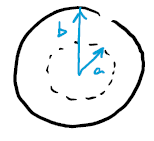
\includegraphics[height=5em]{sph_eg}
    \end{minipage}

    \hfill\\[1em]
    The calculaton of the total mass is then
    \aleq{
        &\int_{r=a}^{r=b}\int_{\phi=0}^{\phi=2\pi}\int_{\theta=0}^{\theta=\pi} \tkn{r4}{\red{\ul{r^4}}} \cdot r^2\sin\theta\dd{\theta}\dd{\phi}\dd{r}\\[1em]
        = &\int_{r=a}^{r=b}\int_{\phi=0}^{\phi=2\pi} \cub[yellow]{\qty(\int_{\theta=0}^{\theta=\pi} r^6\sin\theta\dd{\theta})}{\text{First integrate }\theta}\dd{\phi}\dd{r} \\[1em]
        = &\int_{r=a}^{r=b}\int_{\phi=0}^{\phi=2\pi} \qty[-r^6\cos\theta]\eval_{\theta=0}^{\theta=\pi} \dd{\phi}\dd{r} \\[1em]
        = &\int_{r=a}^{r=b} \cub[blue]{\qty(\int_{\phi=0}^{\phi=2\pi} 2r^6\dd{\phi})}{\text{Then integrate }\phi}\dd{r} \\[1em]
        = &\int_{r=a}^{r=b}\qty[2r^6\phi]\eval_{\phi=0}^{\phi=2\pi} \dd{r} \\[1em]
        = &\cub[green]{\int_{r=a}^{r=b} 4\pi r^6 \dd{r}}{\text{Finally integrate }r} \\[1em]
        = & \frac{4\pi}{7}(b^7-a^7)
    }
    \addArrow[red]{r4}{(4ex, 2ex)}{density function $\rho(r,\theta,\phi)=r^4$}
    {(2ex, 2ex)}{(12ex,1ex)}

\end{example}
%%%
\theend
\end{document}